
% -------------------------------------------------------------------------------------------------------
% Section Single- und Dual-Slope-Wandler

\section{Sigma-Delta-ADC}

\begin{minipage}{0.68\linewidth}
    \begin{tabular}{ll}
        $n$ & Anzahl Bits \\
        $D$ & Digitaler Wert \quad $D < 2^n$ \\
        $q$ & Quantisierungsschritt (1 LSB) \\
        $B_0$ & Bitwert 0 (LSB) \\
        $B_{n-1}$ & Bitwert $n-1$ (MSB)
    \end{tabular}
\end{minipage}
\hfill
\begin{minipage}{0.3\linewidth}
    $ \boxed{ q = \frac{V_{\rm refp} - V_{\rm refn}}{2^n} } $ \\
    $ \boxed{ D = \frac{V_{\rm in} - V_{\rm refn}}{V_{\rm refp} - V_{\rm refn}} \, 2^n }  $
\end{minipage}


\subsection{Dual-Slope-Wandler}

\begin{minipage}{0.42\linewidth}
    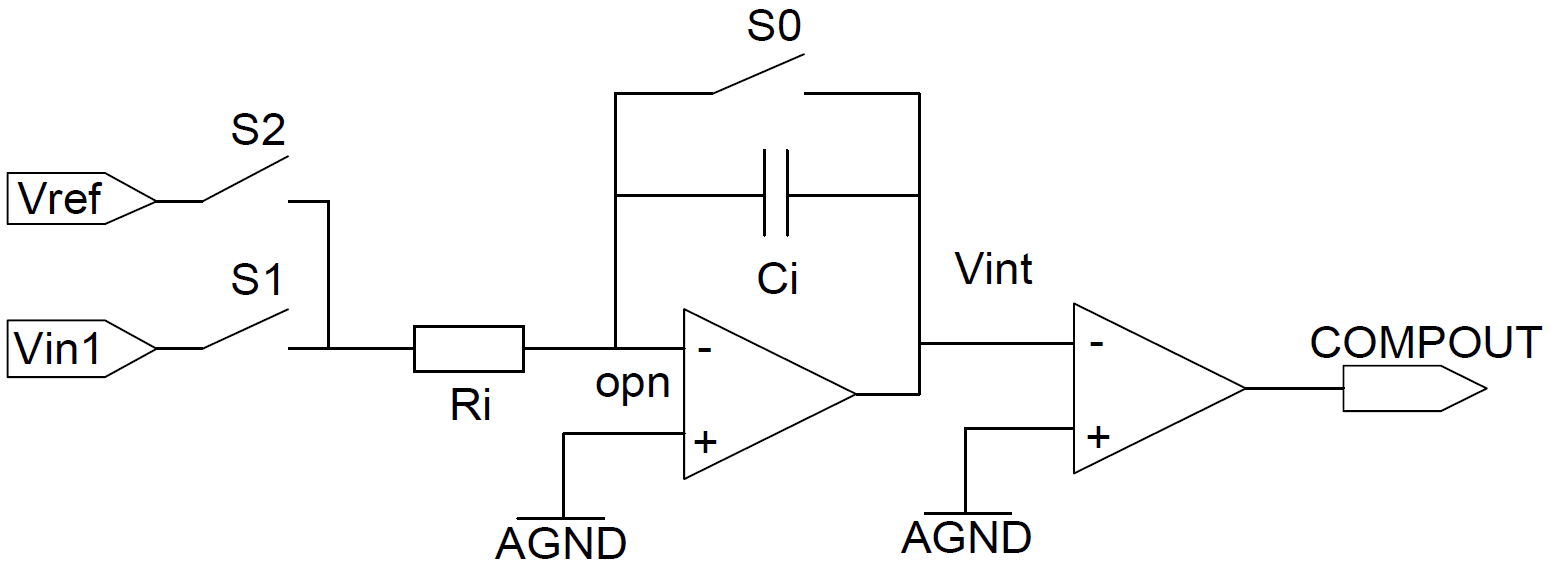
\includegraphics[width=\linewidth]{images/dual_slope_ADC}
\end{minipage}
\hfill
\begin{minipage}{0.27\linewidth}
    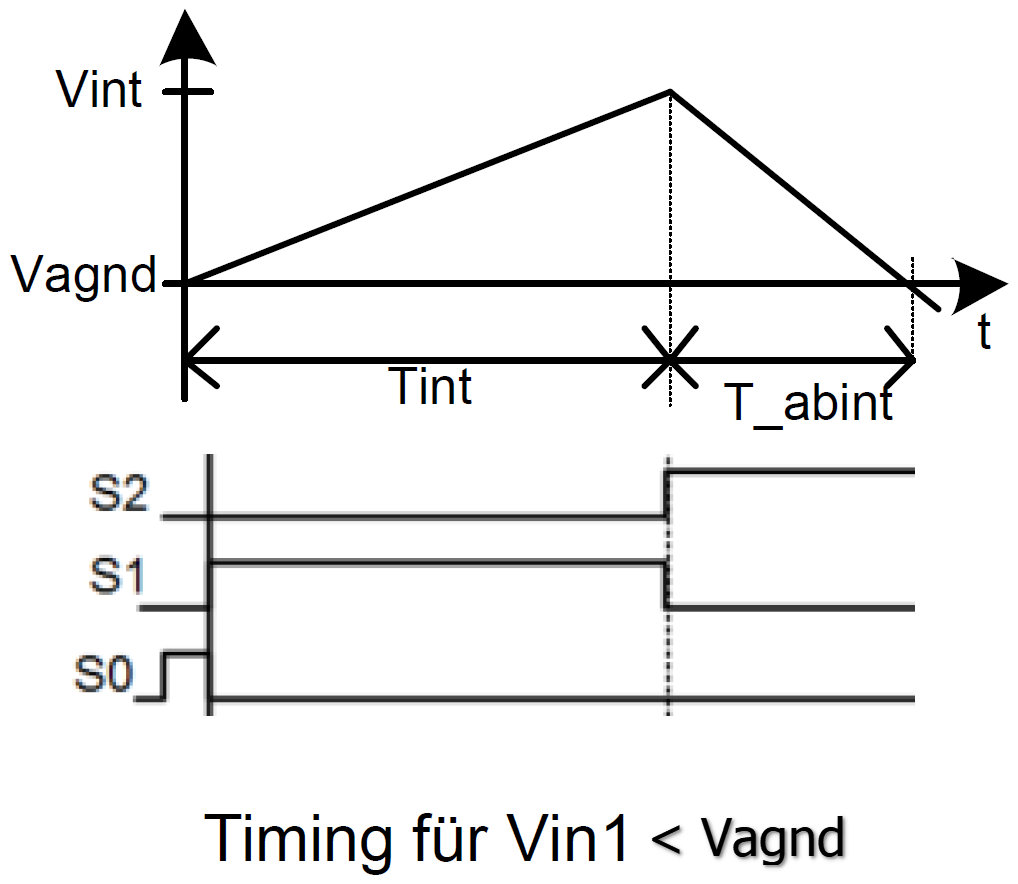
\includegraphics[width=0.83\linewidth]{images//dual_slope_ADC_timing}
\end{minipage}
    \hfill
\begin{minipage}{0.29\linewidth}
    $ \boxed{  V_{\rm int} = \frac{\overline{V_{\rm in}} \cdot T_{\rm int}}{R_i \cdot C_i} } $ 
    $ \boxed{  V_{\rm abint} = \frac{V_{\rm ref} \cdot T_{\rm abint}}{R_i \cdot C_i}  } $ 
\end{minipage}
    
$ \boxed{ \text{DC: } V_{\rm int} = V_{\rm AGND}- \frac{1}{R_i \cdot C_i} \, (V_{\rm in1}- V_{\rm AGND}) \cdot T_{\rm int} } $ 
\quad $\boxed{ \Delta V_{\rm abint} = - \Delta V_{\rm int} }$ \\
$ \boxed{ \Delta V_{\rm abint} = V_{\rm AGND} - V_{\rm int} = - \frac{1}{R_i \cdot C_i} \, (V_{\rm ref} - V_{\rm AGND}) \cdot T_{\rm abint} }$ 
\quad $\boxed{ T_{\rm abint} = - \frac{V_{\rm in1} \cdot T_{\rm int}}{V_{\rm ref}} }$\\
  
$\boxed{\text{Allgemein: } V_{\rm int} = \int\limits_0^{T_{\rm int}} - \frac{1}{R_i \cdot C_i} \, V_{\rm in1} \, \diff t + V_{\rm int,0} }$
\quad 
$ \boxed{ -\frac{\overline{V_{\rm in}}}{V_{\rm ref}}= \frac{T_{\rm abint}}{T_{\rm int}} = \frac{n \cdot T_{\rm clk}}{N \cdot T_{\rm  clk} } }$


\subsubsection{Frequenzverhalten vom Dual-Slope-Wandler}

Frequenzen $f = \frac{1}{T}$ , wobei $T$ der Intergrationszeit entspricht, werden perfekt unterdrückt \\
$\Rightarrow$ Integrationszeit $T = 20 \, \mathrm{ms}$ unterdrückt Netzbrumm von $50 \, \mathrm{Hz}$


% weglassen?
\subsection{Single-Slope-Wandler}

\begin{minipage}[c]{0.52\columnwidth}
    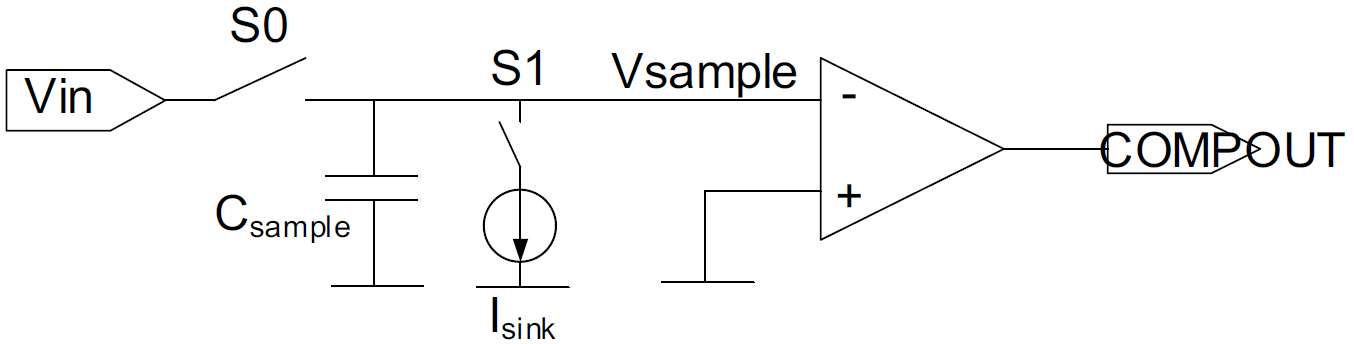
\includegraphics[width=\columnwidth]{images/single-slope-wandler.png}
\end{minipage}
\hfill
\begin{minipage}[c]{0.38\columnwidth}
    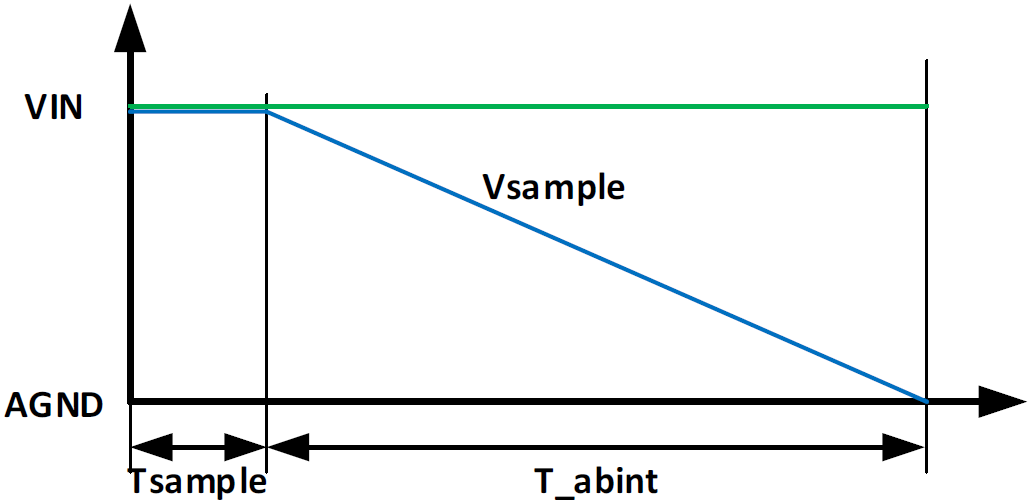
\includegraphics[width=\columnwidth]{images/single-slope-wandler_timing.png}
\end{minipage}

\begin{minipage}[t]{0.48\columnwidth}
    \begin{itemize}
        \item Einfacher als Dual-Slope
        \item $V_ {\rm in}$ wird auf $C_{\rm sample}$ übertragen
        \item $C_{\rm sample}$ wird mit $I_{\rm sink}$ entladen
        \item Zeit bis $V(C_{\rm sample}) = 0$ wird gemessen
    \end{itemize}
\end{minipage}
\hfill
\begin{minipage}[t]{0.48\columnwidth}
    \begin{itemize}
        \item[+] Kein OpAmp, nur zwei Schalter
        \item[+] Schnell, da $T_{\rm sample} < T_{\rm int}$
        \item[-] $V_{\rm in} \sim T_{\rm abint}, \, C_{\rm sample}, \, I_{\rm sink}$
        \item[-] $C_{\rm sample}$ und $I_{\rm sink}$ streuen stark
    \end{itemize}
\end{minipage}


\subsection{Dual-Slope-Wandler für pos. und neg. Eingangsspannungen}

\begin{minipage}[c]{0.52\columnwidth}
    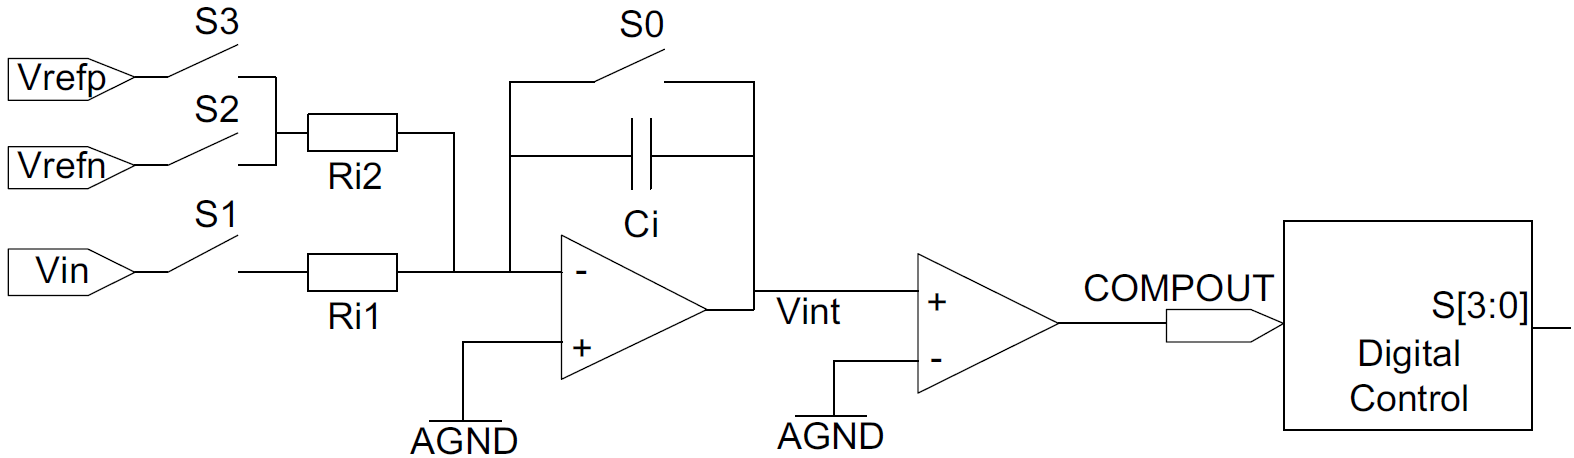
\includegraphics[width=\columnwidth]{images/dual_slope_ADC_pos_neg.png}
\end{minipage}
\hfill
\begin{minipage}[c]{0.37\columnwidth}
    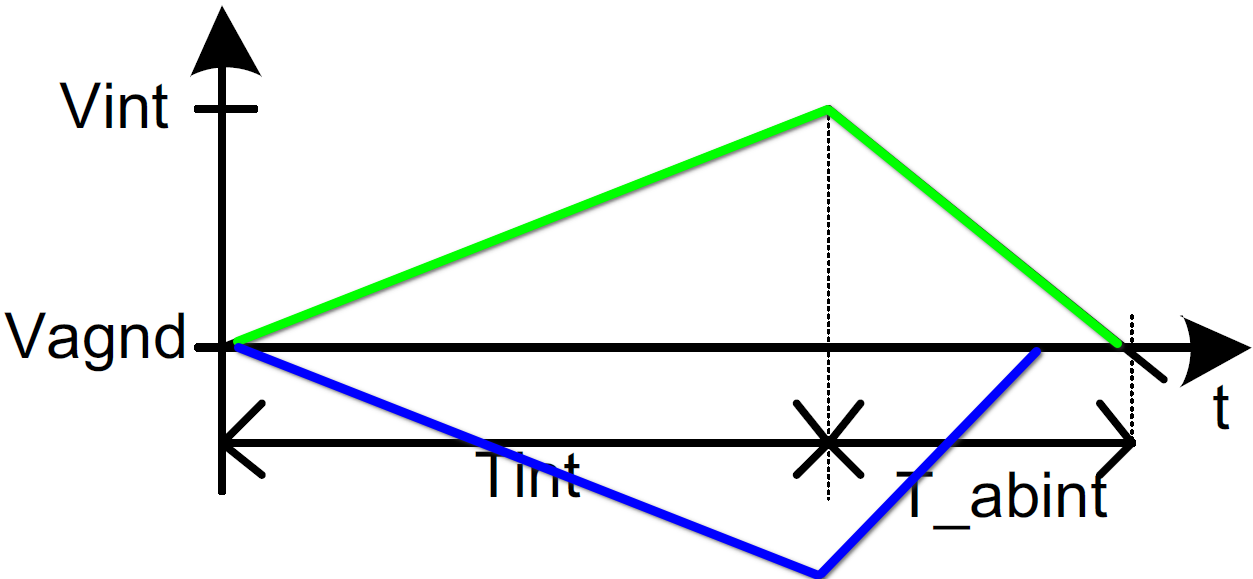
\includegraphics[width=\columnwidth]{images/dual_slope_ADC_pos_neg_timing.png}
\end{minipage}

\begin{minipage}[t]{0.48\columnwidth}
    \begin{itemize}
        \item Auf- und Abintegration wechseln ab
        \item Je nach Komparator-Ausgang wird S2 oder S3 geschlossen
    \end{itemize}
\end{minipage}
\hfill
\begin{minipage}[t]{0.48\columnwidth}
    \begin{itemize}
        \item Für \cgn{$V_{\rm in} < V_{\rm AGND}$} wird in richtung positive Speisung integriert
        \item Für \cbl{$V_{\rm in} > V_{\rm AGND}$} wird in richtung GND integriert
    \end{itemize}
\end{minipage}


\subsubsection{Eigenschaften von Dual-Slope-Wandlern}

\begin{minipage}[t]{0.48\columnwidth}
    \begin{itemize}
        \item Unabhängig von Bauteiltoleranzen
        \item Höhere Auflösung bedingt längere Integrationszeit (bei fixem clk) 
            \textrightarrow\ Doppelte Zeit für 1 zusätzliches Bits
    \end{itemize}
\end{minipage}
\hfill
\begin{minipage}[t]{0.48\columnwidth}
    \begin{itemize}
        \item Höhere Frequenzen werden stärker unterdrückt \textrightarrow\ reduziert Bandbreite
        \item Auflösung wird gegen Bandbreite getauscht
    \end{itemize}
\end{minipage}

% -------------------------------------------------------------------------------------------------------
% \section{Sigma-Delta-ADC}

\subsection{Aufbau Sigma-Delta-ADC}
\label{Aufbau Sigma-Delta-ADC}

\begin{minipage}[t]{0.6\columnwidth}
    \begin{center}
        \myul{Sigma-Delta-ADC}
    \end{center}
    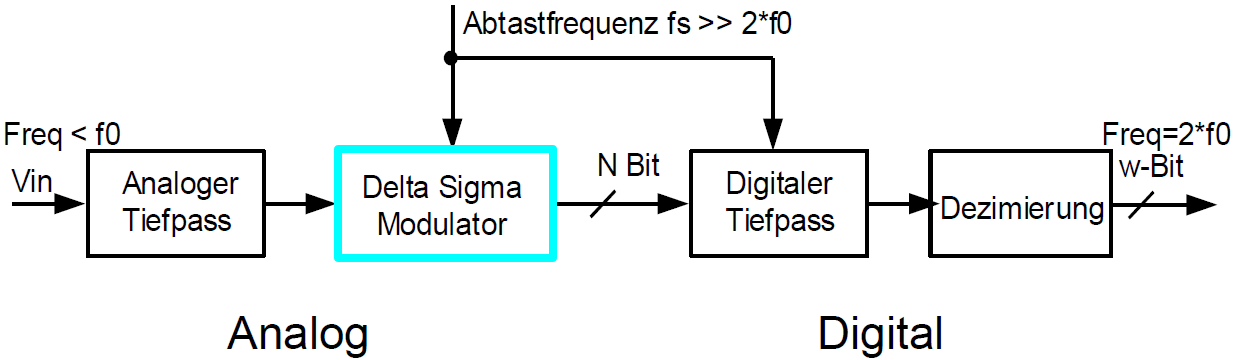
\includegraphics[width=\columnwidth]{images/aufbau_sigma_delta_ADC.png}
\end{minipage}
\hfill
\begin{minipage}[t]{0.38\columnwidth}
    \begin{center}
        \myul{Detail: Sigma-Delta-Modulator}
    \end{center}
    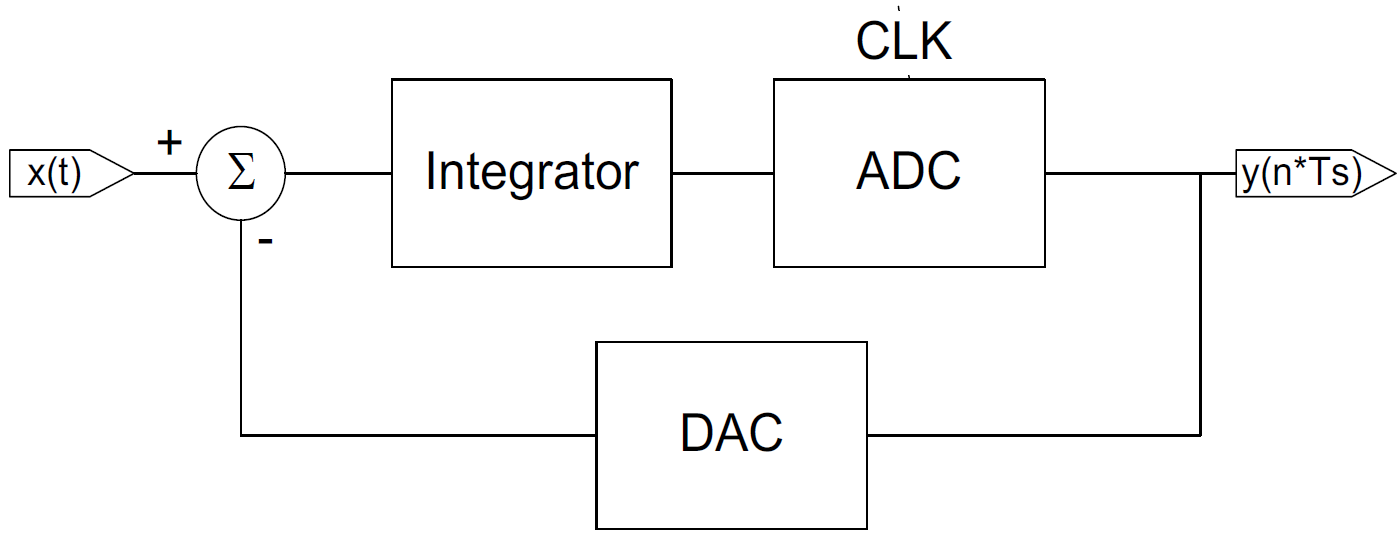
\includegraphics[width=\columnwidth]{images/aufbau_sigma_delta_modulator.png}
\end{minipage}


\subsection{Sigma-Delta-Modulator 1. Ordnung}
\label{Sigma-Delta-modulator Ordnung 1}

\begin{minipage}[c]{0.48\columnwidth}
    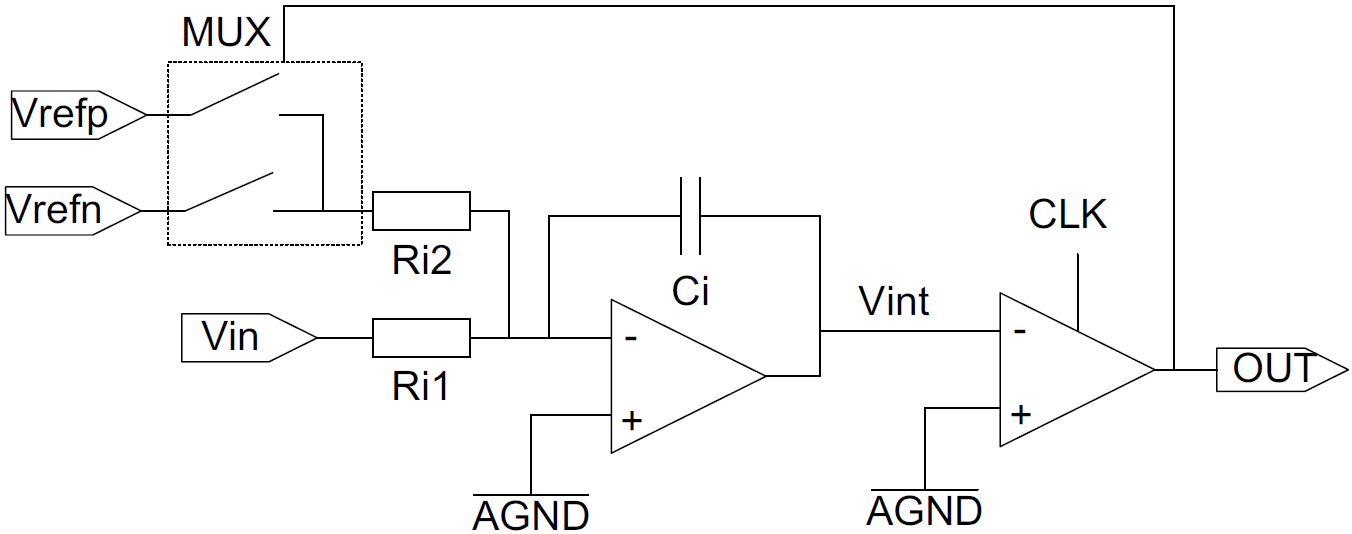
\includegraphics[width=\columnwidth]{images/sigma-delta-wandler.png}
\end{minipage}
\hfill
\begin{minipage}[c]{0.48\columnwidth}
    $$ \boxed{V_{\rm in} = \frac{2 \cdot n  - N}{N} V_{\rm ref}} $$

    \begin{tabular}{ll}
        $N$ & \# Taktzyklen von Clk \\
        $n$ & \# Taktzyklen, in denen \\
            & Modulator-Ausgang $=1$
    \end{tabular}
\end{minipage}
$$\boxed{\text{Allgemein: } V_{\rm int}(t) = \Delta V_{\rm int} + V_{\rm int,0} 
    = - \frac{1}{C_i} \int\limits_0^{t} \Bigg( \frac{V_{\rm in} - A_{ \rm GND}}{R_{i1}} + \frac{V_{\rm ref} - A_{ \rm GND}}{R_{i2}} \Bigg) \diff \tilde{t} + V_{\rm int,0} }$$

\begin{itemize}
    \item Sigma-Delta-Wandler machen \textbf{gleichzeitig} Auf- und Abintegration (Feedback-Pfad)
    \item 'Digitales Filter' \textrightarrow\ 'Mittelwertbildung' um $V_{\rm in}$  zu berechnen
    \item Eingangsspannungsbereich: $V_{\rm refn} \leq V_{\rm in} \leq V_{\rm refp}$ \textrightarrow\ $I_{\rm Eingang} \leq I_{\rm Feedback}$
    \item \textbf{Summe aller Ladungen muss gesamthaft 0 sein!} \textrightarrow\ $\Delta Q = C \cdot \Delta U = I \cdot \Delta t = 0$
\end{itemize}


\subsection{Sigma-Delta-Modulator im Zeitbereich}

\subsubsection{DC-Eingangssignale}

\begin{minipage}[c]{0.6\columnwidth}
    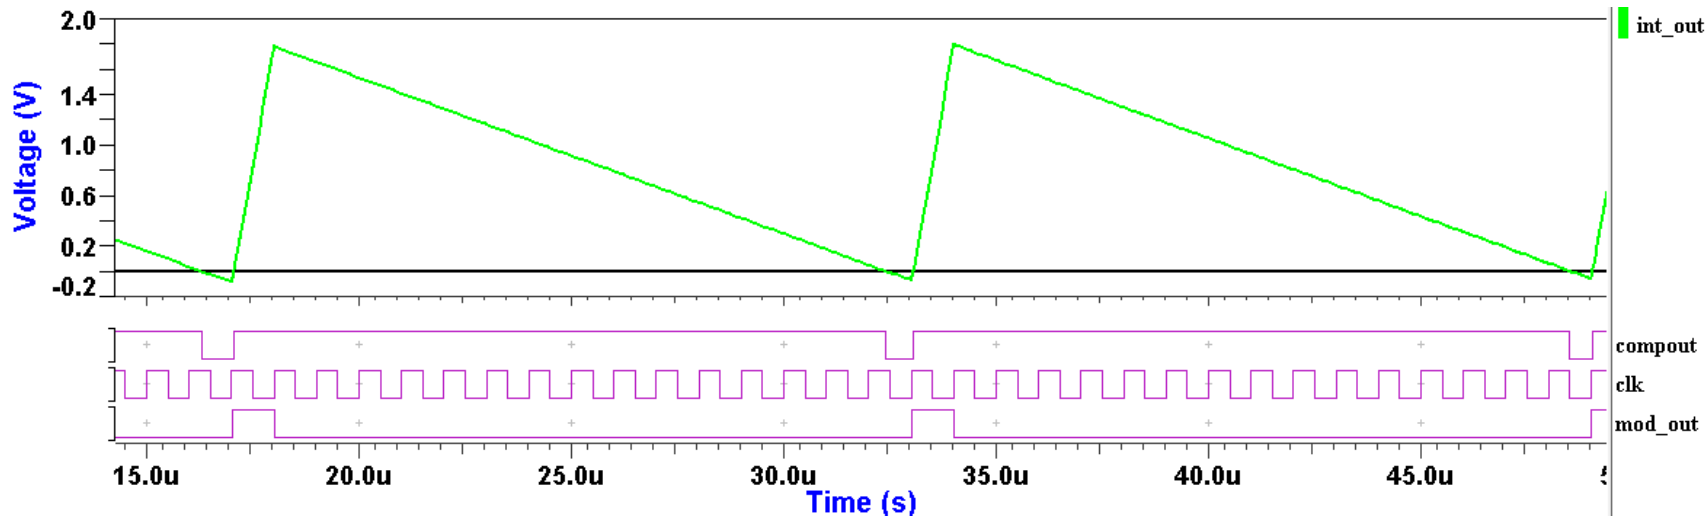
\includegraphics[width=\columnwidth]{images/sigma_delta_timing.png}

    Je nach $V_{\rm in}$ ergibt sich ein anderer DutyCycle $\frac{n}{N}$\\
    (mod out). Für $V_{\rm refn} = - V_{\rm refp}$ gilt die aufgeführte Tabelle. 
\end{minipage}
\hfill
\begin{minipage}[c]{0.38\columnwidth}
    \begin{tabular}{c | c}
        $\bf{V_{\rm in}}$               & \textbf{Duty Cycle} $\bf{\frac{n}{N}}$ \\
        \midrule
        $0 \, \volt$                    & $\frac{1}{2}$ \\
        $\frac{1}{2} \, V_{\rm refn}$   & $\frac{1}{4}$ \\
        $\frac{7}{8} \, V_{\rm refn}$   & $\frac{1}{16}$ \\
        $\frac{1}{10} \, V_{\rm refp}$  & $\frac{11}{20}$ \\
        $0.02 \cdot \, V_{\rm refp}$    & $\frac{51}{100}$
    \end{tabular}
\end{minipage}


\subsubsection*{Fazit DC-Eingangssignale}

\begin{itemize}
    \item DC-Eingangssignale erzeugen \textbf{repetitive Sequenzen} mit hohen Frequenz-Anteilen
    \item Ist $V_{\rm in}$ nahe bei Bruchteil vin $V_{\rm ref}$ entstehen \textbf{lange repetitive Sequenzen} mit tiefen Frequenz-Anteilen
    \item \textbf{Lange repetitive Sequenzen können nicht von Signal unterschieden werden\\
        \textrightarrow\ Pattern Noise}
\end{itemize}
        

\subsubsection{AC-Eingangssignale}

AC-Eingangssignale können durch Mittelwertbildung (z.B. mit Tiefpassfilter mit entsprechend hoch dimensinierter Zeitkonstante) 
des Signals $V_{\rm int}$ rekonstruiert werden.




\subsection{Modellierung Sigma-Delta-Modulator im Frequenzbereich}

\begin{minipage}[c]{0.4\columnwidth}
    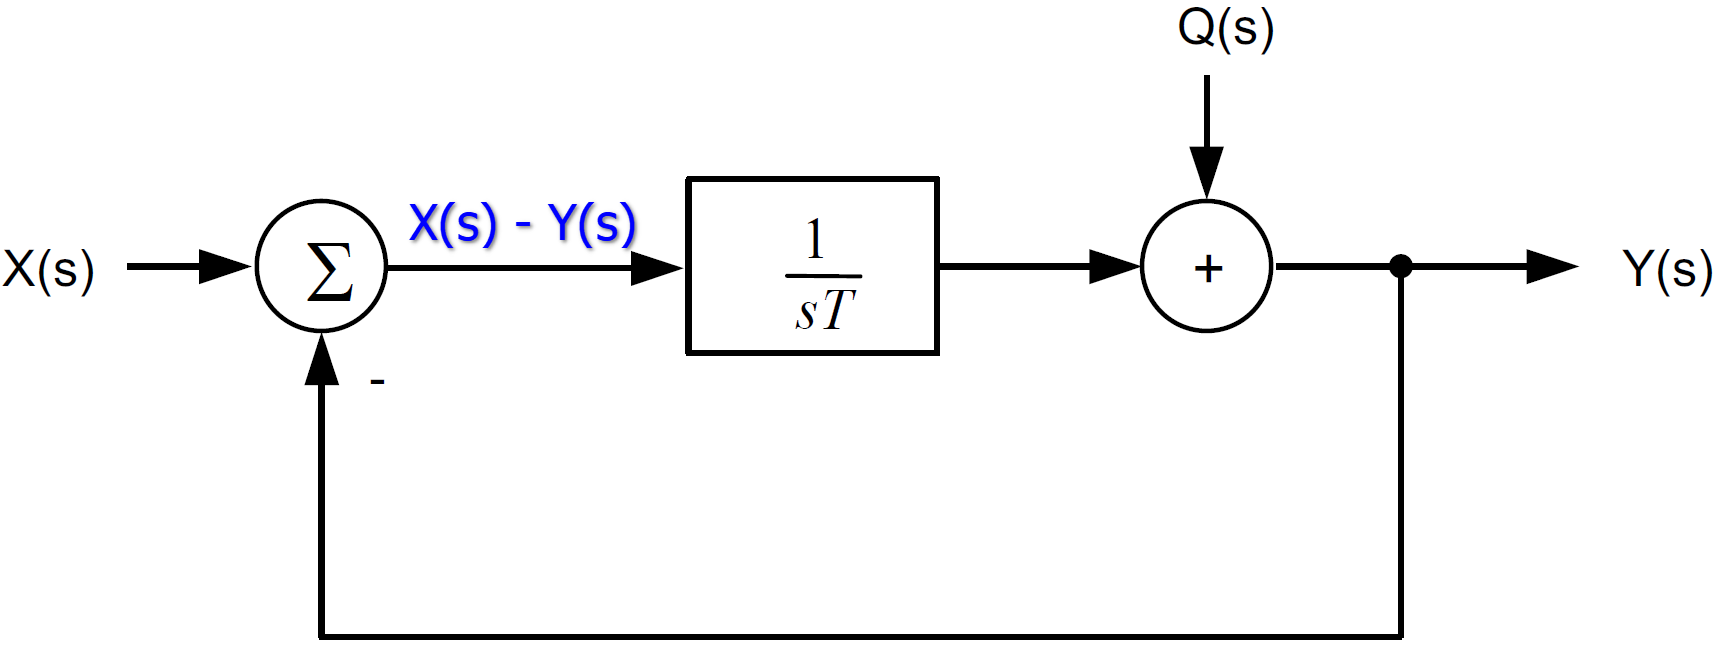
\includegraphics[width=\columnwidth]{images/sigma-delta-modulator_frequenzbereich.png}
\end{minipage}
\hfill
\begin{minipage}[c]{0.58\columnwidth}

    \begin{tabular}{ll}
        $Q(s)$          & Quantisierungsrauschen \\
        $A_{\rm ADC}$   & Verstärkungsfaktor ADC ($=1$) \\
        $A_{\rm DAC}$   & Verstärkungsfaktor DAC ($=1$) 
    \end{tabular}
\end{minipage}


\subsubsection{Übertragungsfunktionen Sigma-Delta Modulator}

\begin{minipage}[t]{0.48\columnwidth}
    \begin{center}
        \myul{Signal-Übertragungsfunktion $H_s(s)$}
        (Quantisierungsrauschen $Q(s) = 0$)
    \end{center}
    $$ Y(s) = [X(s) - Y(s)] \cdot\frac{1}{s \cdot T} $$
    $$ \boxed{ H_s(s) = \frac{Y(s)}{X(s)} = \frac{1}{1 + s \cdot T} \quad \text{(Tiefpass)}} $$
\end{minipage}
\hfill
\begin{minipage}[t]{0.48\columnwidth}
    \begin{center}
        \myul{Noise-Übertragungsfunktion $H_n(s)$}
        (Eingangssignal $X(s) = 0$)
    \end{center}
    $$ Y(s) = - Y(s) \cdot\frac{1}{s \cdot T} + Q(s) $$
    $$ \boxed{ H_n(s) = \frac{Y(s)}{Q(s)} = \frac{s \cdot T}{1 + s \cdot T} \quad \text{(Hochpass)}} $$
\end{minipage}

% gutes Bild für Noise-Übertragungsfunktion bzw. Noise-Shaping aber ka wohin damit
% 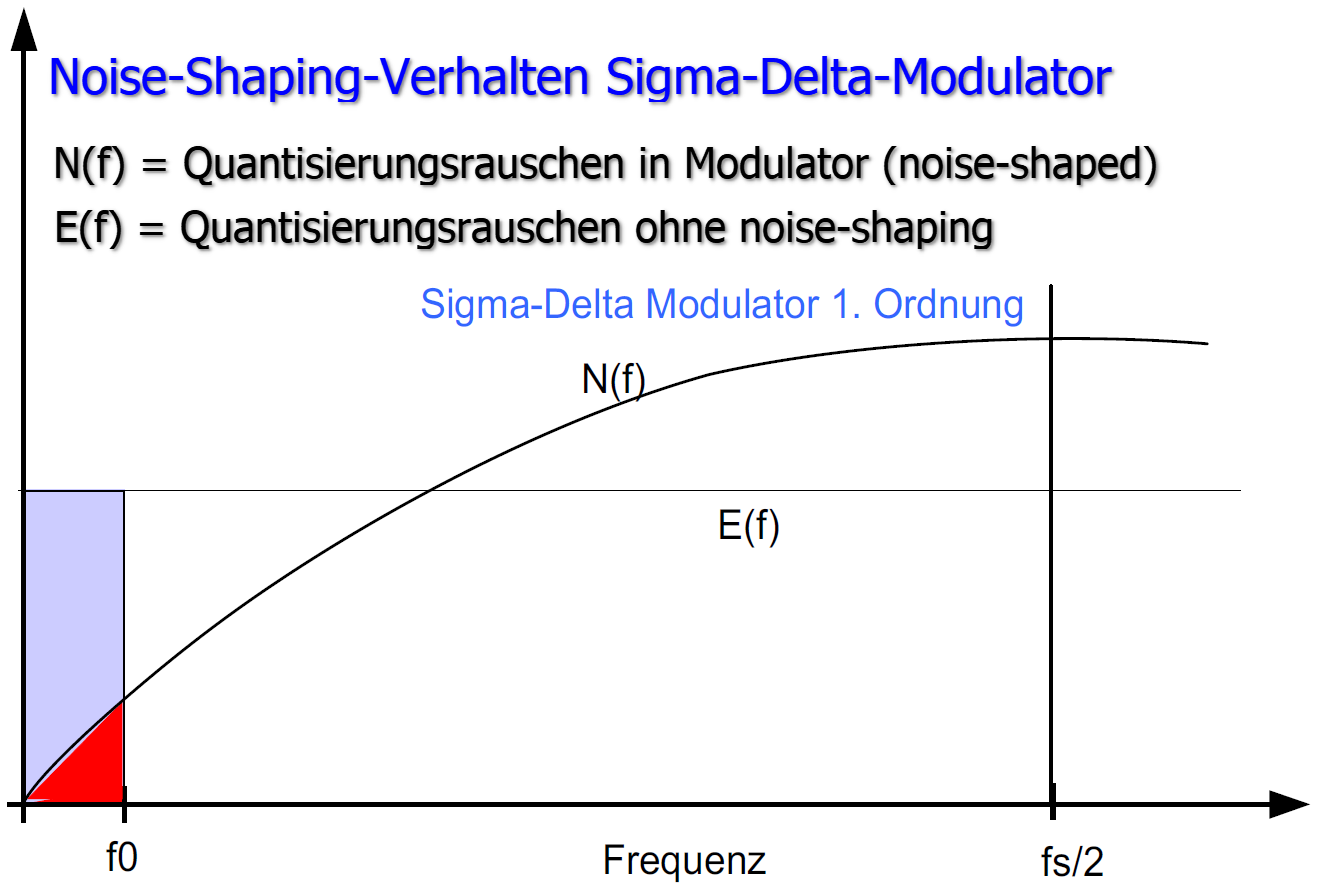
\includegraphics[width=\columnwidth]{images/noise_shaping_sigma_delta.png} 


\subsection{Oversampling / Signal-Rausch-Abstand (SNR)}

$$ \boxed{ \text{Rauschleistung} = \text{Rauschleistungsdichte} * \text{Bandbreite} = \frac{q^2}{12} = \text{konstant}} $$

\begin{itemize}
    \item Oversampling verteilt Quantisierungsrauschen über grösseren Frequenzbereich
    \item Da die Rauschleistung konstant ist, wird die Rauschleistungsdichte (also die 'Amplitude' des Rauschens) kleiner
    \item Ein Digitalfilter reduziert die Bandbreite des ADCs weiter
\end{itemize}

\begin{minipage}[c]{0.48\columnwidth}
    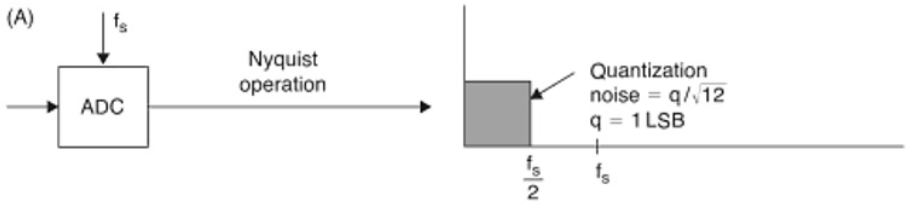
\includegraphics[width=\columnwidth]{images/rauschen_ohne_oversampling.png}
\end{minipage}
\hfill
\begin{minipage}[c]{0.48\columnwidth}
    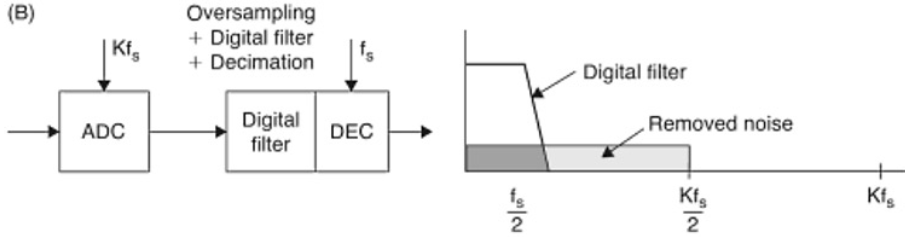
\includegraphics[width=\columnwidth]{images/rauschen_mit_oversampling.png}
\end{minipage}


\subsubsection{Noise-Shaping}

\begin{minipage}[c]{0.48\columnwidth}
    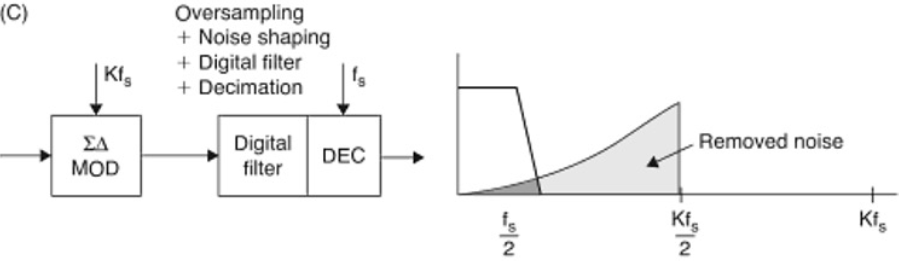
\includegraphics[width=\columnwidth]{images/rauschen_mit_oversampling_und_noise_shaping.png}
\end{minipage}
\hfill
\begin{minipage}[c]{0.48\columnwidth}
    \begin{itemize}
        \item Nicht nur Oversampling und Rauschen gleichmässig verteilen, sondern Rauschleistungsdichte 'formen'
        \item \textbf{Nur bei Sigma-Delta-Wandlern möglich}
    \end{itemize}
\end{minipage}


\subsection{Sigma-Delta-Wandler 2. Ordnung}

\begin{minipage}[c]{0.48\columnwidth}
    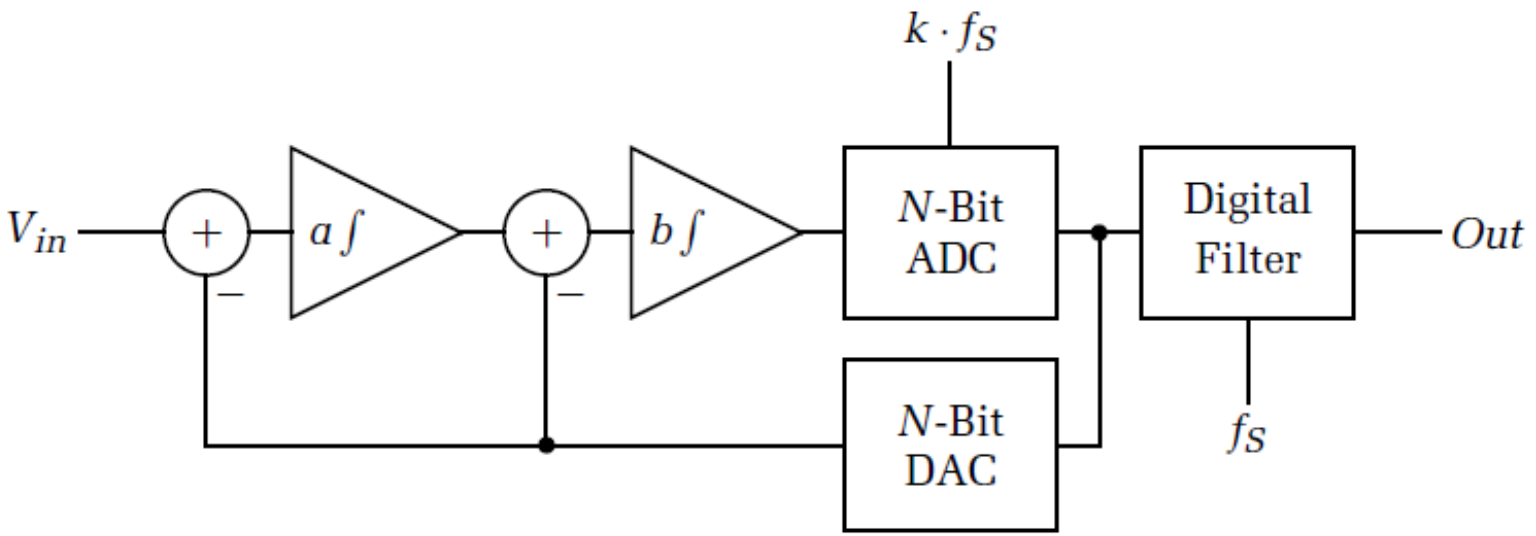
\includegraphics[width=\columnwidth]{images/sigma-delta-wandler_ordnung_2.png}
\end{minipage}
\hfill
\begin{minipage}[c]{0.48\columnwidth}
    $$ \boxed{ \text{SNR} \approx \log_{10} \Bigl( \frac{3}{2} \cdot \frac{2 \cdot M + 1}{\pi^{2M}} \cdot \text{OSR}^{2M+1} \Bigr) } $$
    \begin{tabular}{ll}
        OSR & Oversampling-Rate \\
        $M$ & Ordnung des Modulators
    \end{tabular}
\end{minipage}

\begin{itemize}
    \item Ordnung $M = 2$ \textrightarrow\ 2 Integratoren
    \item Quantisierungsrauschen $Q(s)$ wird mit Hochpass 2. Ordnung gefiltert
    \item Je höher Ordnung $M$, desto stärker das Noise-Shaping ($6 \, \deci \bel$ pro Ordnung und Oktave)
    \item Je höher Oversampling (OSR), desto höher SNR ($3 \, \deci \bel$ Oktave)
\end{itemize}


% ------------------------------------------------------------------------------------------------------------------------------------
% \section{Multi-Bit Modulatoren}
\subsection{Multi-Bit Modulatoren}

Anstatt eines Komparators ADCs mit mehreren Bits für den Aufbau des Sigma-Delta-\textbf{Modulators} verwendet.

\begin{minipage}[t]{0.48\columnwidth}
    \begin{itemize}
        \item[+] \textbf{Dynamikgewinn von ca. $\bm{6 \, \deci \bel }$ pro zusätzlichem Bit.}
    \end{itemize}
\end{minipage}
\hfill
\begin{minipage}[t]{0.48\columnwidth}
    \begin{itemize}
        \item[-] Aufwändiger Flash-ADC (parallele Komparatoren) nötig, da in einem Takt gewandelt werden muss
    \end{itemize}
\end{minipage}


% weglassen? von Slides abgeschrieben...
\subsection{1 Bit vs. Multi-Bit ADC (im Modulator)}

\begin{itemize}
    \item ADC ist unproblematisch, da hinter Integrator (siehe Blockschaltbild Abschnitt~\ref{Aufbau Sigma-Delta-ADC}) und dahei 
        Teil vom Quantisierungsfehler
    \item 1-Bit ADC (Komparator) nichtlinear \textrightarrow\ ADC-Verstärkung signalabhängig
    \item Es entsteht ein nichtlineares System
\end{itemize}


% weglassen? von Slides abgeschrieben...
\subsection{1 Bit vs. Multi-Bit DAC (im Modulator)}

\begin{outline}
    \1 DAC muss volle Präzision des (gesamten) Wandlers haben
        \2 DAC-Spannung wird direkt mit Eingangsspannung 'verrechnet'
    \1 1-Bit DAC ist perfekt linear (nur Offset- und Gain-Fehler, welche statisch kompensierbar sind)
    \1 DAC muss sehr genau sein \textrightarrow\ kann kalibriert werden
        \2 Drifttemperatur und Alterung sind dennoch ein Problem
\end{outline}


\subsection{Dynamic Element Matching (DEM), Mismatch-Shaping}

\begin{minipage}[c]{0.4\columnwidth}
    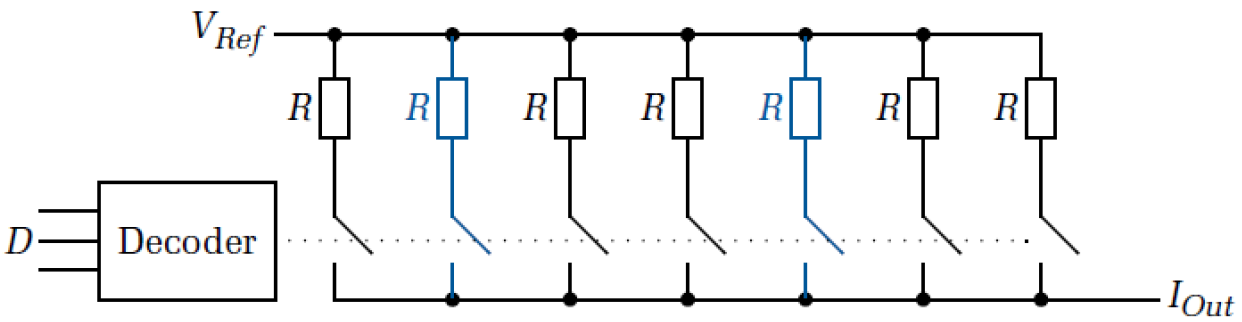
\includegraphics[width=\columnwidth]{images/strom-DAC.png}
\end{minipage}
\hfill
\begin{minipage}[c]{0.58\columnwidth}
    \begin{outline}
        \1 Widerstände des DAC müssen perfekt matchen (so gut wie DAC-Genauigkeit)
            \2 In der Praxis ist das nicht möglich!\\
                \textrightarrow\ mismatch
    \end{outline}
\end{minipage}

\vspace{0.2cm}

\begin{outline}
    \1 Dynamic Element Matching (DEM): Spezieller Algorithmus
        \2 Einschalten der einzelnen Widerstände wird dynamisch umgestaltet, so dass Ausgangskennline des DAC 
            'durchschnittlich linear' \\
            \textrightarrow\ Systematischer Fehler wird in Zufallsfehler (Rauschen) umgewandelt
    \1 Mismatch-Shaping 
        \2 Zufallsfehler (Rauschen) wird mit Noise-Shaping gedämpft
\end{outline}


\subsection{Fazit Sigma-Delta-Modulatoren}

\begin{minipage}[t]{0.48\columnwidth}
    \begin{itemize}
        \item[+] Signal wird nicht (wenig) verändert mit Tiefpass
        \item[+] 1 Bit DAC perfekt linear 
        \item[+] 1. SNR-Erhöhung durch Oversampling ($3 \, \deci \bel$ pro Oktave)
        \item[+] 2. SNR-Erhöhung durch Noise Shaping ($6 \, \deci \bel$ pro Oktave)
        \item[+] 3. SNR-Erhöhung durch ADC/DAC im Modulator ($+6 \, \deci \bel$ pro Bit)
    \end{itemize}
\end{minipage}
\hfill
\begin{minipage}[t]{0.48\columnwidth}
    \begin{itemize}

        \item[+] Modulatoren 1. Ordnung immer stabil ($90 \degree$ Phasenschiebung)
        \item[+] Modulatoren 2. Ordnung meistens stabil
        \item[-] Modulatoren höherer Ordnung können instabil werden  
        \item[-] 1 Bit ADC (Komparator) nichtlinear
        \item[-] \textbf{Pattern Noise} 
    \end{itemize}
\end{minipage}


\subsection{Digitalfilter}

Der digitale Teil des Sigma-Delta-ADCs kann auf mehrere Arten realisiert werden.  Das Digitalfilter soll die folgenden Aufgaben
erfüllen:

\begin{minipage}[t]{0.55\columnwidth}
    \begin{itemize}
        \item Reduktion des Rauschens (wegen Noise-Shaping viel Rauschen bei hohen Frequenzen)
    \end{itemize}
\end{minipage}
\hfill
\begin{minipage}[t]{0.42\columnwidth}
    \begin{itemize}
        \item Erhöhung der Auflösung
        \item Redution der Sample Rate
    \end{itemize}
\end{minipage}


\subsubsection{Mittelwertbildung}

Einfachste Mittelwertbildung umgesetzt mittels countern \textrightarrow\ Funktionsweise und Formel 
siehe Abschnitt~\ref{Sigma-Delta-modulator Ordnung 1}


\subsubsection{Kammfilter (Mittelwertfilter)}

\begin{minipage}[t]{0.45\columnwidth}
    \begin{tabular}{ll}
        $Z^{-1}$    & um $1$ Takt verschieben \\
        $Z^{-L}$    & um $L$ Takte verschieben \\
    \end{tabular}
\end{minipage}
\hfill
\begin{minipage}[t]{0.52\columnwidth}
    \begin{tabular}{ll}
        FIR    & Finite Impulse Response \\
        IIR    & Infinite Impulse Response \\
    \end{tabular}
\end{minipage}

\vspace{0.2cm}

\begin{minipage}[t]{0.58\columnwidth}
    \begin{center}
        \myul{FIR-Filter}
    \end{center}
    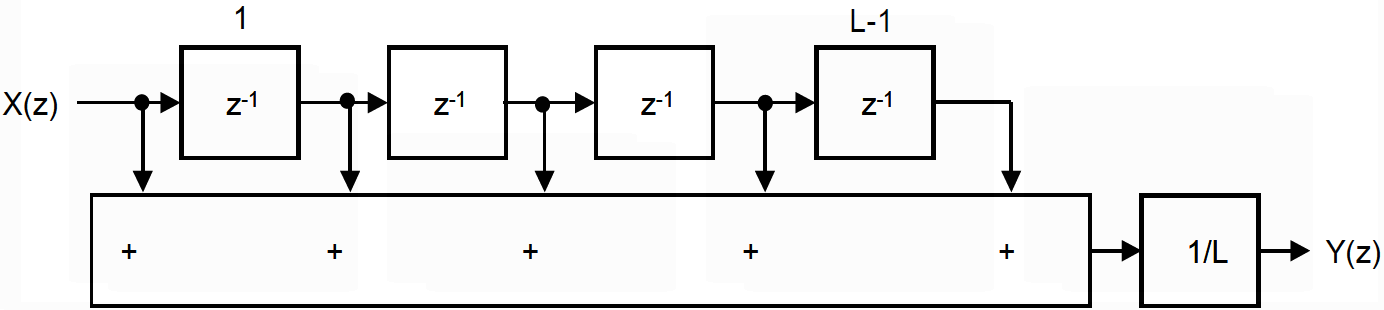
\includegraphics[width=\columnwidth]{images/kammfilter.png}
\end{minipage}
\hfill
\begin{minipage}[t]{0.38\columnwidth}
    \begin{center}
        \myul{IIR-Filter}
    \end{center}
    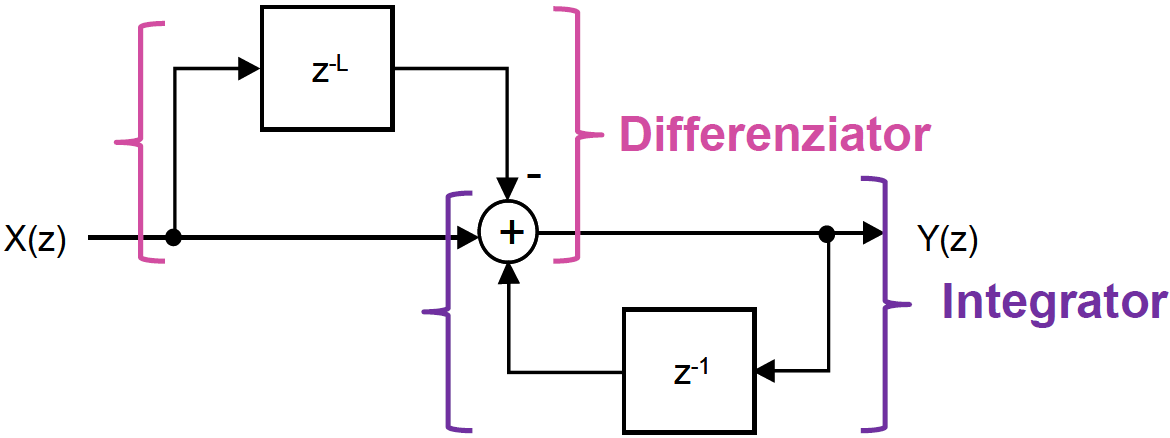
\includegraphics[width=\columnwidth]{images/kammfilter_IIR-filter.png}
\end{minipage}

\subsubsection*{Frequenzgang kaskadierte Kammfilter}

\begin{minipage}[c]{0.4\columnwidth}
    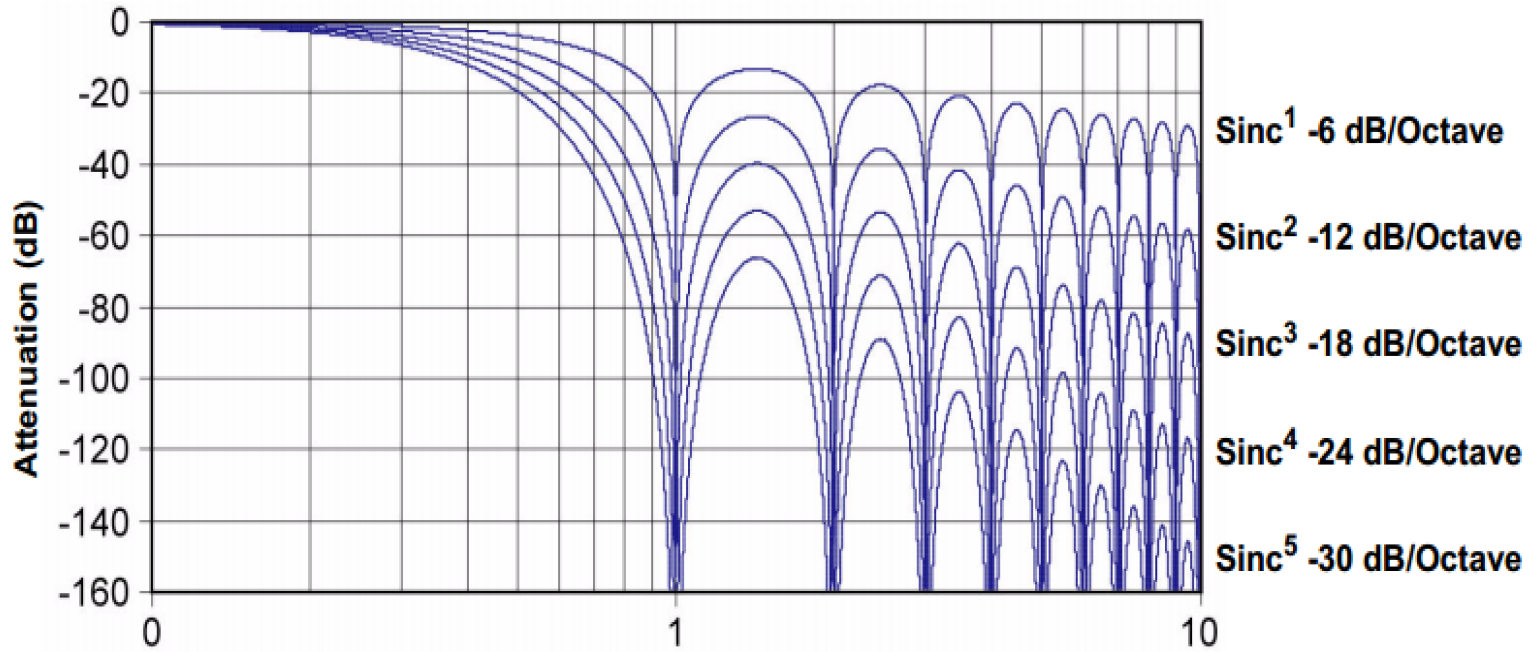
\includegraphics[width=\columnwidth]{images/frequenzgang_kaskadierte_kammfilter.png}
\end{minipage}
\hfill
\begin{minipage}[c]{0.58\columnwidth}
    \begin{itemize}
        \item Bezeichnung kaskadierte Kammfilter: \\
            CIC (Cascaded-Integrator-Comb-Filter)
        \item Notches ('Auslöschungen') bei $n \cdot \frac{\text{Sampling-Freq.}}{L}$
        \item Je höher die Ordnung, desto steiler der Abfall im Amplitudengang
    \end{itemize}
\end{minipage}


\section{Sigma-Delta-DAC}

Die finale Realisierung des DACs erfolgt als \textbf{PWM-DAC}. Die Generierung des PWM-Sigmals erfolgt nach dem Sigma-
Delta-Prinzip

\begin{minipage}[t]{0.58\columnwidth}
    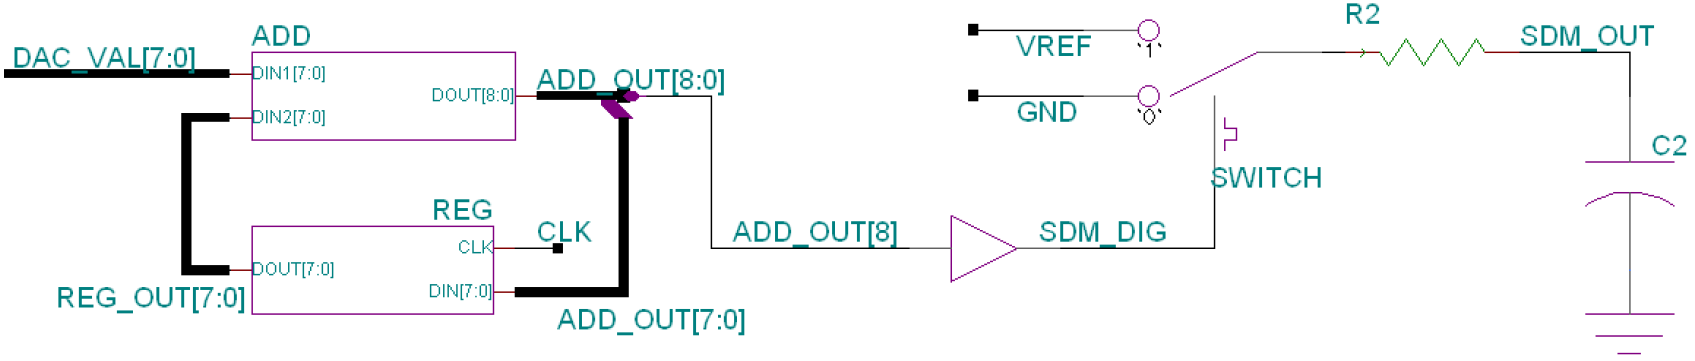
\includegraphics[width=\columnwidth]{images/sigma-delta_DAC.png}
\end{minipage}
\hfill
\begin{minipage}[t]{0.38\columnwidth}
    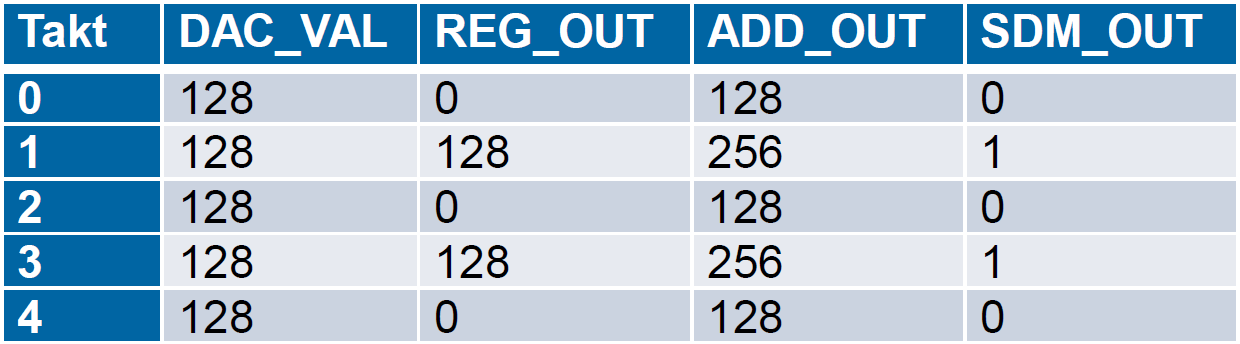
\includegraphics[width=\columnwidth]{images/sigma-delta_DAC_verlauf.png}
\end{minipage}

\subsection{Pattern-Noise}

Für einen 8-Bit DAC ist der digitale Wert $129$ ungünstig, da in der Bitsequenz irgendwann zwei '1' hintereinander auftauchen.
Dies führt zu einer grossen Periodendauer, welche ein \textbf{Pattern Noise} beim DAC verursacht, da die '0' und '1' möglichst
gleichmässig auf die gesamte Periode verteilt werden.




\subsection{Bilanz Sigma-Delta-DAC}

\begin{minipage}[c]{0.48\columnwidth}
    \begin{itemize}
        \item Verhalten wie analoger Modulator (Blockschaltbild)
    \end{itemize}

    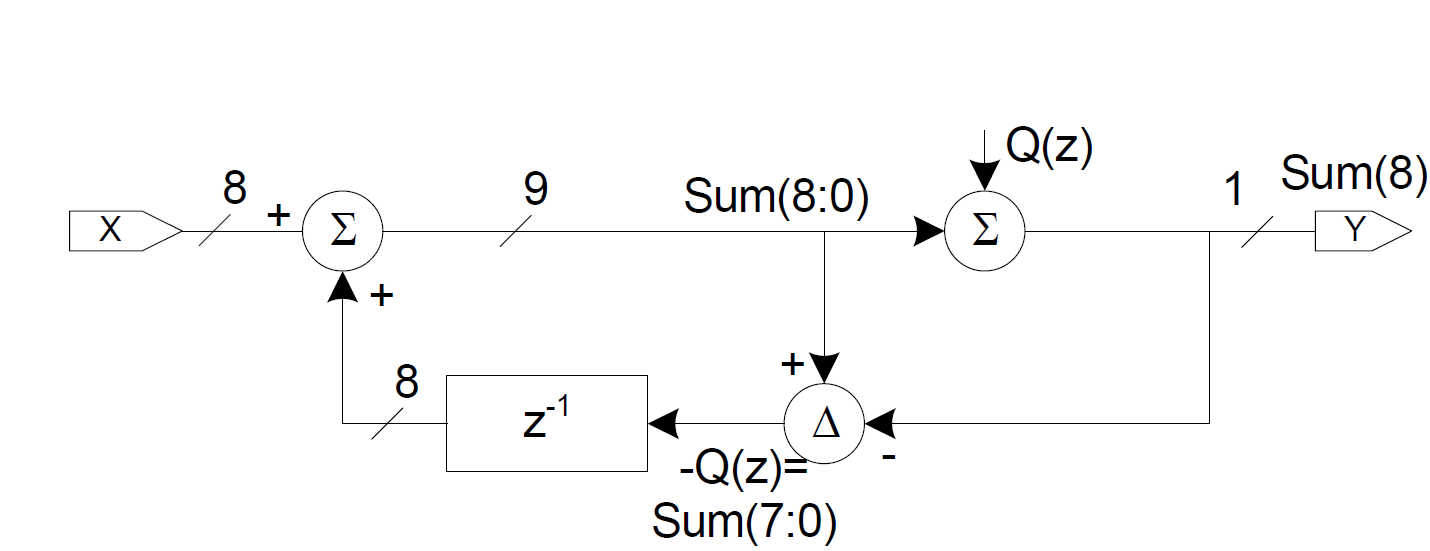
\includegraphics[width=\columnwidth]{images/sigma-delta-DAC_blockschaltbild.png}
\end{minipage}
\hfill
\begin{minipage}[c]{0.48\columnwidth}
    \begin{itemize}
        \item Im Mittel gleich viele '1' und '0' wie bei PWM $= \frac{n}{N}$
        \item '1' werden möglichst gleichmässig in Periode verteilt ($N \cdot T_{\rm clk}$)
        \item Gleichmässige Verteilung ergibt regelmässige Sequenzen \textrightarrow\ periodische Signale \textrightarrow\ unerwünschte
            Frequenzkomponenten (Pattern Noise)
    \end{itemize}
\end{minipage}



